\documentclass[a4paper, 12pt]{report}
\usepackage[a4paper,hmargin={3cm,2.5cm},vmargin={2.5cm,2.5cm}]{geometry}
\usepackage[utf8]{inputenc}
\usepackage{amsmath}
\usepackage{amsfonts}
\usepackage{graphicx}
\usepackage{hyperref}
\usepackage{multicol}
\usepackage{subfig}
\usepackage{float}
\usepackage{xcolor}
\usepackage{blindtext}
\usepackage[english,vietnam]{babel}
\usepackage{fancyhdr}
\pagestyle{fancy}
\lhead{}
\rhead{\nouppercase{\rightmark}}
\renewcommand{\footrulewidth}{1pt}
\usepackage{tikz}
\usetikzlibrary{calc}
\usepackage{eso-pic}
\usepackage{longtable}
\renewcommand{\baselinestretch}{1.2}



\usepackage{minted} % insert code
\usepackage{xcolor}

\begin{document}
\begin{titlepage}
\begin{tikzpicture}[overlay,remember picture]
\draw[line width=4pt]
    ($ (current page.north west) + (1cm,-1cm) $)
    rectangle
    ($ (current page.south east) + (-1cm,1cm) $);
\draw[line width=1.5pt]
    ($ (current page.north west) + (1.2cm,-1.2cm) $)
    rectangle
    ($ (current page.south east) + (-1.2cm,1.2cm) $);
\end{tikzpicture}
%}
\begin{center}
\textup{
\large
\textbf{Viet Nam National University Ho Chi Minh City}\\
\textbf{University of Information Technology}}\\

%---------------------------------Figure------------------------------

\begin{center}
\begin{figure}[htbp]  %h means here other options t , b, p, etc.
\centering

\includegraphics[width=0.3\linewidth]{./logo}
\end{figure}
\end{center}

%----------------------------
\textup{\large  A REPORT ON}\\[0.5cm]
\begin{Large}
{\textbf {SINGULAR VALUE DECOMPOSITION}}\\[0.2cm]
{\textbf{AND PRINCIPAL COMPONENT ANALYSIS}}\end{Large}\\[2cm]
\begin{large}\textup {CS115.L11.KHTN}\end{large}\\[0.5cm]
\textup{SUBMITTED BY}\\[0.3cm]
\begin{large}
\begin{tabular}{ c l }
 19521300 & Cuong Manh Do Nguyen \\
 19520218 & Phu Minh Nguyen  \\  
 19522424 & Trung Huu Le  \\ 
\end{tabular}
\end{large}
\\[1cm]\textup{UNDER THE GUIDANCE OF}\\[0.5cm]
\begin{large}\textbf{Ph.D. HOANG NGOC LUONG}\\[3cm]\end{large}
\textbf{Ho Chi Minh City, January 2021}
\vfill
\end{center}
\end{titlepage}
%================end of title page======================
\setcounter{page}{1}
\newpage
\tableofcontents

\newpage
\chapter{\Large Singular Value Decomposition (SVD)}
\indent \par In Linear Algebra, we learned about diagonalization: a square matrix $A \in R^{n\times n}$ is diagonalizable if exist an invertible matrix $P$ and a diagonal matrix $D$ so that:
 $$ \mathbf{A} = \mathbf{P} \mathbf{D} \mathbf{P}^{-1} $$
But it only happens in the square matrix, not all kinds of the matrix. So \textbf{Singular Value Decomposition} (SVD) is a \textbf{\textit{special matrix factorization}} method for \textit{any} real matrix, which helps us a lot in working with matrix and big data: storing matrix, finding features in data reduction, dimensional reduction, etc. It's considered as a foundation of Machine Learning, one of the most useful tools in numerical linear algebra numerical for data processing. It's also the basis of Principal Component Analysis (PCA) - a wide technique for analyzing high dimensional data. SVD is the basis of the facial recognition algorithm.
\section{Introduction to SVD}
The singular value decomposition of a matrix is usually referred to as the SVD.
This is the final and best factorization of any matrix:
$$\mathbf{A}_{m \times n} = \mathbf{U}_{m \times m}\mathbf{\Sigma}_{m \times n} (\mathbf{V}_{n \times n})^T  ~~~~~(1)$$
where $U$ is \textbf{orthonormal},  $\Sigma$ is almost a \textbf{diagonal} matrix - only contains real numbers ordered \textbf{descending} $\sigma_{1,2,....m}$ in main \textbf{diagonal} line ,$V$ is also \textbf{orthonormal}.\\

\begin{figure}[H]
    \center
    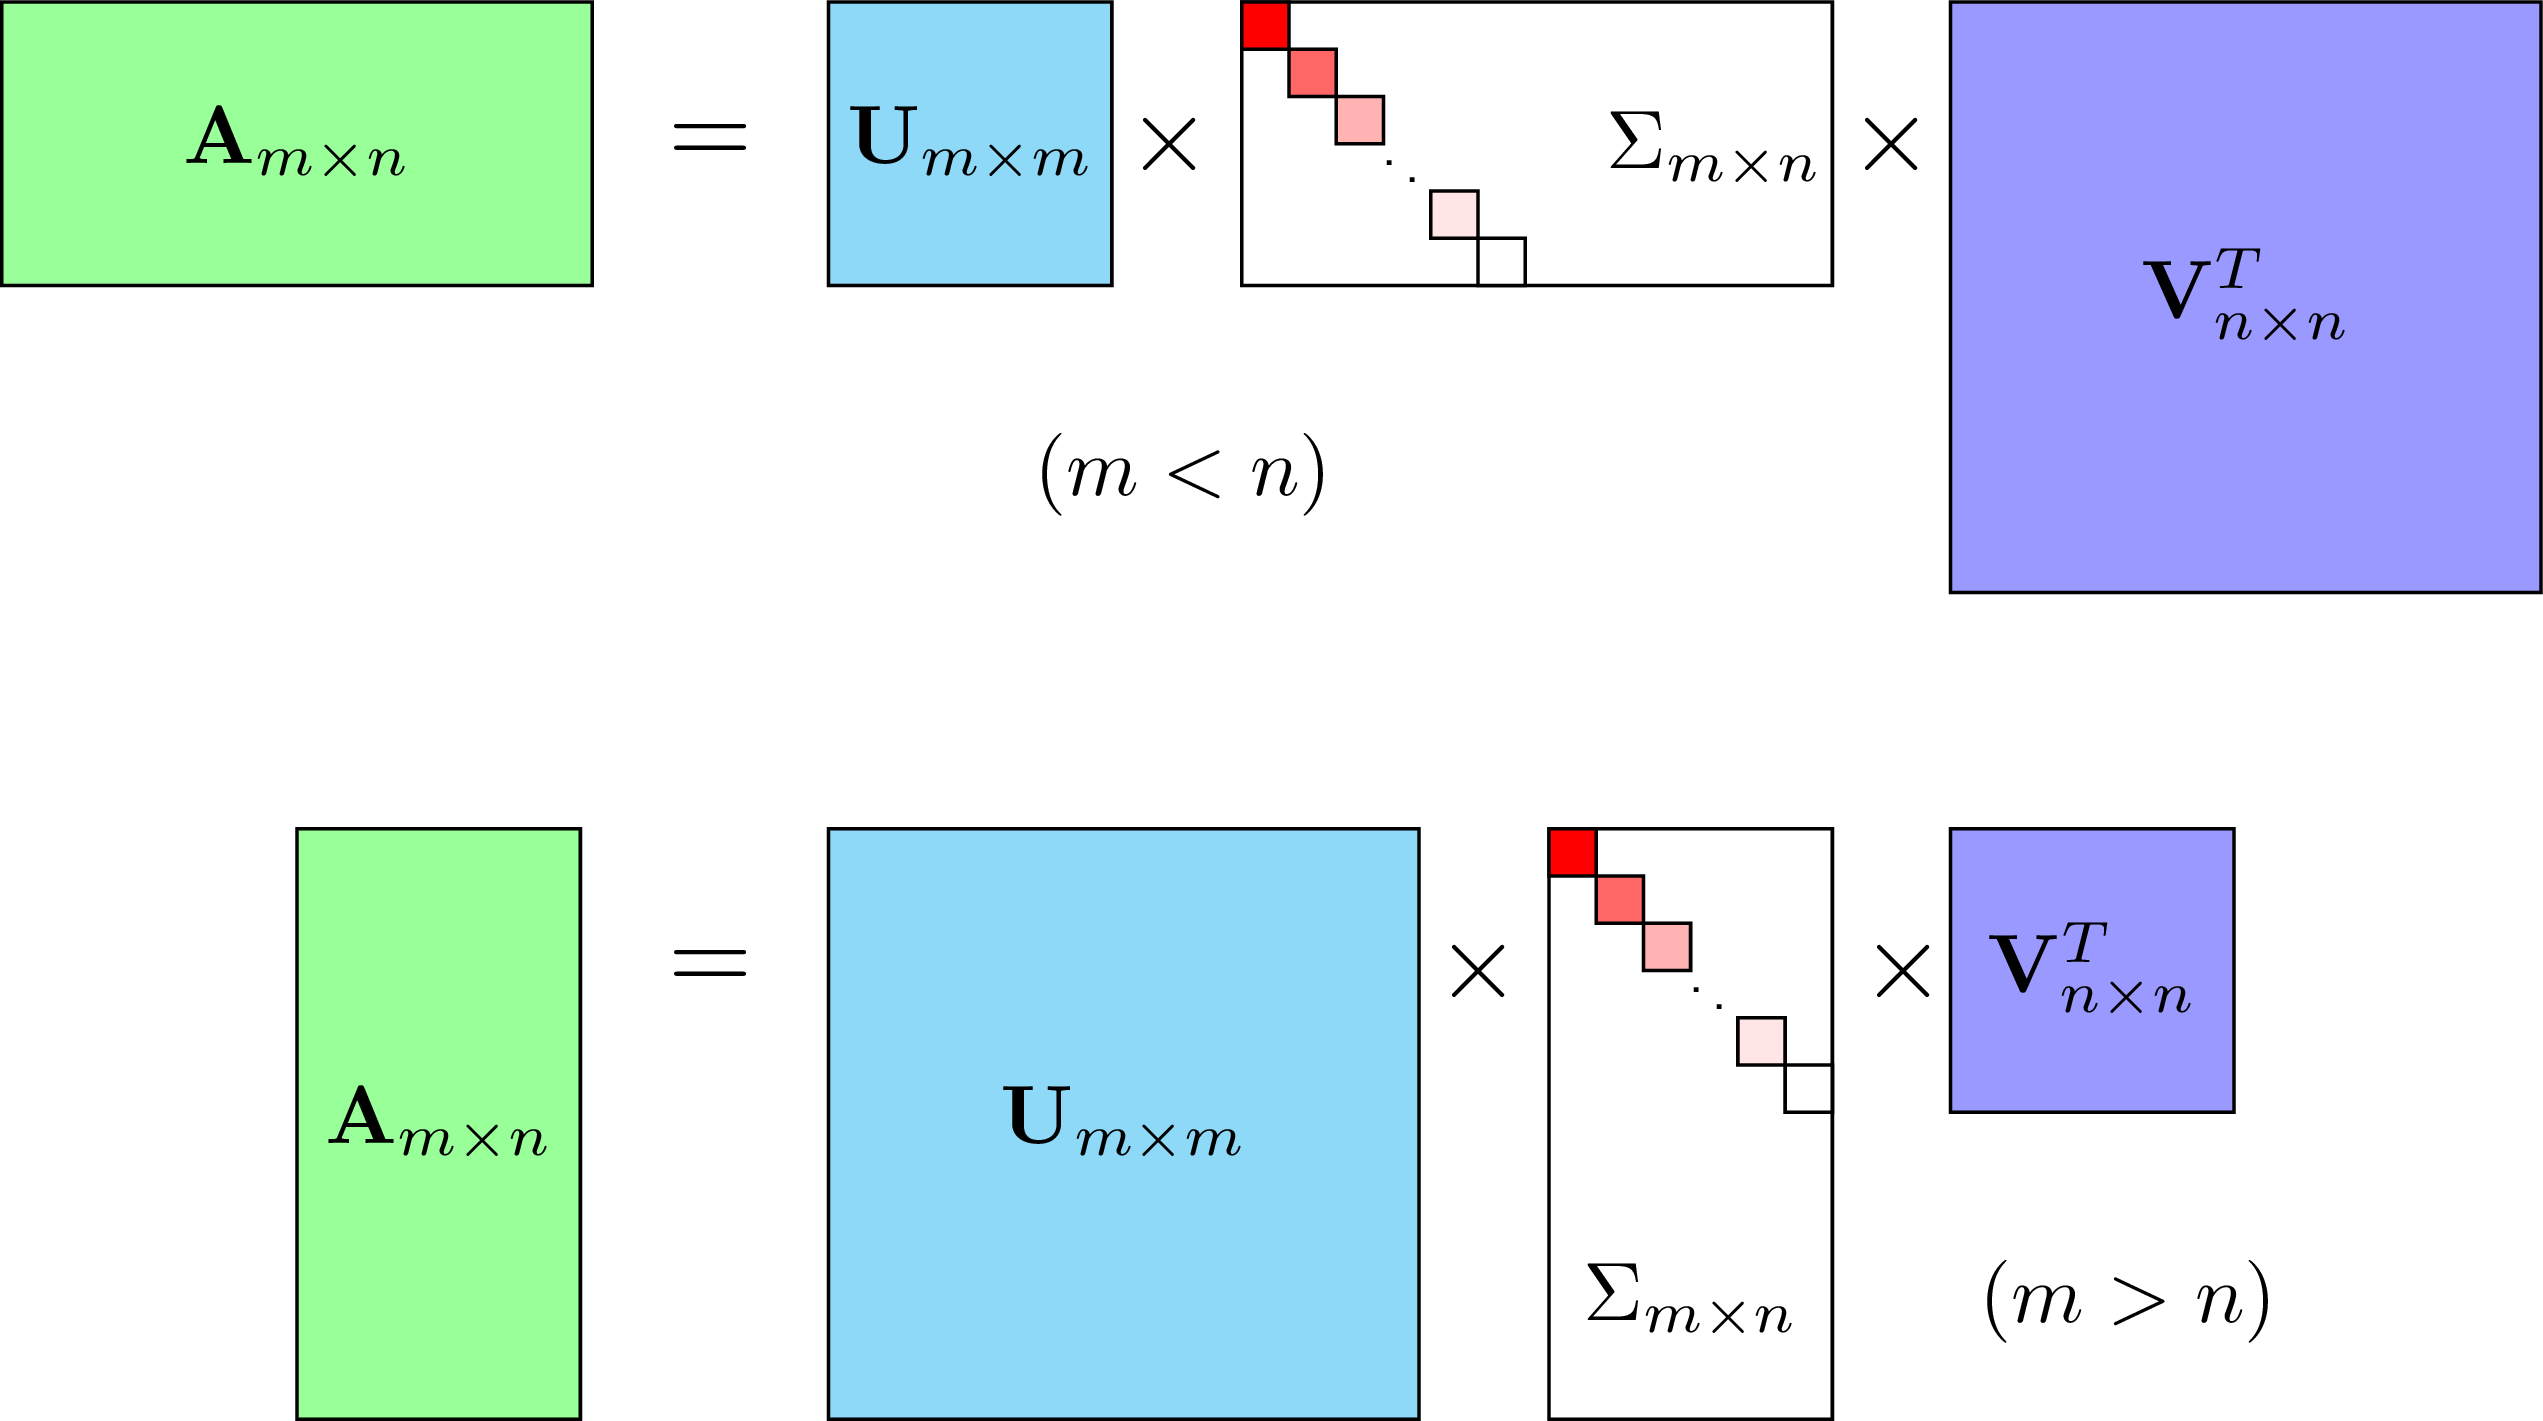
\includegraphics[width=10cm,height=5cm]{svd.png}
    \caption{The image describes the SVD for matrix A in 2 cases: $m < n $ and $m > n$}
\end{figure}
\section{Math Revision}
\subsection{Orthogonal matrix and orthonormal vector}
\begin{itemize}
    \item We say that 2 vectors are orthogonal if they are non-zero vectors and perpendicular to each other. i.e their dot product equal to zero.  For example, $u$ and $v$ are orthogonal if $u^Tv = 0$.
    \item We say that a set of vectors $\{\vec{u_1}, \vec{u_2},...,\vec{u_n}\}$ is mutually orthogonal if every pair of vectors is orthogonal.
    \item 2 vectors are orthonormal if they are orthogonal and their magnitude equal to $1$.
    \item A set of vectors $\{\vec{u_1}, \vec{u_2},...,\vec{u_n}\}$ is orthonormal if every pair of vectors is orthonormal. i.e.
\end{itemize}
    \begin{equation*}
      u_i^Tu_j = 
      \begin{cases}
        1, & i = j \\
        0, & i \neq j
      \end{cases}
    \end{equation*}
\subsection{Gram - Schmidt Algorithm }
\indent \par For a set of linearly independent vectors $\{\vec{v_1}, \vec{v_2},...,\vec{v_n}\}$ $\in$ $\mathbb{R}^n$, we can construct an orthonormal set of vectors:
 \begin{itemize}
  \item Let $u_1 = \frac{v_1}{\lVert v_1 \rVert}$

  \item For $i = 2$ to $n$:
    * Orthogonalization: $u_i = v_i - (u_{i-1}^Tv_i)u_{i-1} - ... - (u_1^Tv_i)u_1$
    
    \item Normalization: $u_i = \frac{u_i}{\lVert u_i \rVert}$
\end{itemize}
\indent \par For example: Matrix $A =\begin{pmatrix}
  1 & 1\\
  1 & -1
  \end{pmatrix}
  $with a set of vectors $a_1 = \begin{bmatrix}1\\1\end{bmatrix}$ and $a_2 = \begin{bmatrix}1\\-1\end{bmatrix}$
\begin{itemize}
  
  
  \item Check independently matrix: $det(A) = -2 \neq 0$
  
  \item Let $u_1 = \frac{a_1}{\lVert a_1 \rVert} = \begin{bmatrix} \frac{1}{\sqrt{2}} \\ \frac{1}{\sqrt{2}} \end{bmatrix}$
 
  \item $i = 2$:
  $u_2 = a_2 - (u_1^Ta_2)u_1 = \begin{bmatrix} 1 \\ -1 \end{bmatrix}$
 
  \item $u_2 = \frac{u_2}{\lVert u_2 \rVert} = \begin{bmatrix} \frac{1}{\sqrt{2}} \\ \frac{-1}{\sqrt{2}} \end{bmatrix}$
\end{itemize}  
\indent \par So matrix $A$ after orthonormalization:
  $A = \begin{pmatrix}
  \frac{1}{\sqrt{2}} & \frac{1}{\sqrt{2}}\\
  \frac{1}{\sqrt{2}} & \frac{-1}{\sqrt{2}}
  \end{pmatrix}$

\section{Calculating SVD}
\indent \par Ignoring dimension of the matrix, base on equation $(1)$ we can compute $AA^T$ like this:
\begin{equation*}
\mathbf{AA}^T = \mathbf{U}\mathbf{\Sigma} \mathbf{V}^T (\mathbf{U}\mathbf{\Sigma} \mathbf{V}^T)^T  
= \mathbf{U}\mathbf{\Sigma} \mathbf{V}^T \mathbf{V}\mathbf{\Sigma}^T\mathbf{U}^T
= \mathbf{U}\mathbf{\Sigma}\mathbf{\Sigma}^T\mathbf{U}^T = \mathbf{U}\mathbf{\Sigma}\mathbf{\Sigma}^T\mathbf{U}^{-1}  ~~~~~ (2)
\end{equation*}
\indent \par $\Sigma \Sigma^T$ is a diagonal matrix contains $\sigma^2_{1},\sigma^2_{2}...\sigma^2_{m}$. These $\sigma^2$ is eigenvalues of $AA^T$ and its is not negative. Those $\sigma_j$ is square root of $AA^T$ eigenvalues - also called as \textbf{singular values}. Column vectors of $U$ are eigenvectors of $AA^T$. We call these vectors are \textbf{left-singular vectors}.\\
\indent \par In the other hand, calculating $A^TA$ will look like this:
\begin{equation*}
\mathbf{A}^T\mathbf{A} = (\mathbf{U}\mathbf{\Sigma} \mathbf{V}^T)^T \mathbf{U}\mathbf{\Sigma} \mathbf{V}^T 
= \mathbf{V}\mathbf{\Sigma}^T\mathbf{U}^T   \mathbf{U}\mathbf{\Sigma} \mathbf{V}^T 
= \mathbf{V}\mathbf{\Sigma}^T\mathbf{\Sigma}\mathbf{V}^T =  \mathbf{V}\mathbf{\Sigma}^T\mathbf{\Sigma}\mathbf{V}^{-1} ~~~~~ (3)
\end{equation*}

Similar to $AA^T$, column vectors of $V$ are eigenvectors of $A^TA$. We call these vectors are \textbf{right-singular vectors}.

\par\textbf{Prove eigenvalues of $A^T A$ and $A A^T$ are the same:}
\par Let $\lambda \ne 0$ be an eigenvalue of $A^T A$ with corresponding eigenvector $ \mathbf v \ne \mathbf 0$ :
\begin{eqnarray*}
 \Rightarrow A^T A \mathbf v &=& \lambda \mathbf v\\
 \Leftrightarrow AA^T A \mathbf v &=& \lambda A \mathbf v \\
 \Leftrightarrow AA^T \mathbf u &=& \lambda u ~~~(u=Av)
\end{eqnarray*}
\par $\lambda$ is an eigenvalue of $A A^T$ as well, with eigenvector $\mathbf u = A \mathbf v$.
\par Now show that if $\lambda$ s eigenvalue for $AA^T$ with corresponding eigenvector $\mathbf u \ne \mathbf 0$
\begin{eqnarray*}
 \Rightarrow AA^T\mathbf u &=& \lambda \mathbf u\\
 \Leftrightarrow A^TAA^T \mathbf u &=& \lambda A^T \mathbf u \\
 \Leftrightarrow A^TA \mathbf z  &=& \lambda \mathbf z ~~~(z=A^Tu)
\end{eqnarray*}

\textbf{So eigenvalues of $A^T A$ and $A A^T$ are the same! $(4)$}\\
From $(2)(3)(4)$, we can get matrix $\Sigma, U , V$ just by diagonalizing $A^TA$ or $AA^T$.\\
Image depicting the transfer facility in svd:
\begin{figure}[H]
    \center
    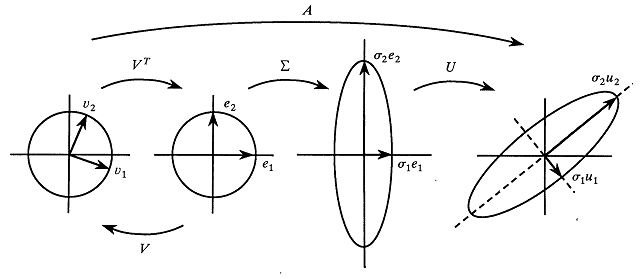
\includegraphics[width=10cm,height=5cm]{svdcs.png}
\end{figure}

\section{Some special SVD}
\indent \par In reality, data is very complex, and it can be lots of entries and features. For example, human genetic data can be a sequence of thousand features, and there are thousands of people - which is huge; finding "eigenface" of people for facial recognition, a grey picture contains 1 face, may have a size 400 x 400 pixel, having different lighting condition, enormous data like that can't be interpreted and analyzed. Even though, after doing SVD with these data, it's still large. Truncated SVD will help us solve this big data problem. We will store a part of the origin SVD, but still knowing the main features.
\subsection{Compacted SVD}
\indent\par Equation $(1)$ can be written as below:
  $$ \mathbf{A} = \sigma_1 \mathbf{u}_1 \mathbf{v}^T_1 + \sigma_2\mathbf{u}_2\mathbf{v}_2^T + \dots + \sigma_r\mathbf{u}_r\mathbf{v}_r^T $$
\indent with every $u_i v_i^T, 1 \leq i \leq r$ is a rank-1 matrix.\\
\indent \par In this formula, $A$ only depends on \textbf{first r columns} of $U$, \textbf{first r rows} of $V$ and \textbf{r} values in main diagonal line of $\Sigma$. So we have a better decomposition called \textbf{compacted SVD}:
$$ \mathbf{A} = {\mathbf{U}}_r{\Sigma}_r({\mathbf{V}}_r)^T $$
If our $A$ has a smaller rank than \textbf{columns and rows} of $A$, meaning $ r \ll m,n$. Therefore, we have the benefit of compacted SVD in storing data.
\subsection{Truncated SVD}
\indent \par Remembered, $\sigma$ values in the main diagonal line of $\Sigma$ is non-zero and ordered descending. In common, some first values of $\sigma_i$ are large, remaining values are small and can be zero. We do not want to store all the values in the SVD. Then, we can approximate matrix  $A \approx \hat{A} $ equal to sum of $k$ ($< r$) rank-1 matrices:
$$\mathbf{A} \approx \mathbf{\hat{A} } = U_k \Sigma_k V_k^T = \sigma_1 \mathbf{u}_1 \mathbf{v}^T_1 + \sigma_2\mathbf{u}_2\mathbf{v}_2^T + \dots + \sigma_k\mathbf{u}_k\mathbf{v}_k^T $$
Pushing away $r-k$ small and non-zero values in \textbf{SVD} is called \textbf{Truncated SVD}. The error of subtraction $A-A_k$ is calculated by the Frobineous norm of the subtraction. But we have a theorem for it. \textbf{The error will equal to total square of the cut-off eigenvalues in truncated SVD}.
$$||\mathbf{A} - \mathbf{A}_k||_F^2 = \sum_{i = k + 1}^r \sigma_i^2 ~~~(5)$$
\indent\par Proof:
\indent\par\begin{eqnarray*}
    ||\mathbf{A} - \mathbf{A}_k||_F^2 &=& ||\sum_{i = k + 1}^r \sigma_i \mathbf{u}_i\mathbf{v}_i^T ||_F^2  ~~~~~~~ (6) \\
    &=& \text{trace}\left\{ \left(\sum_{i = k + 1}^r \sigma_i \mathbf{u}_i\mathbf{v}_i^T\right)
    \left(\sum_{j = k + 1}^r \sigma_j \mathbf{u}_j\mathbf{v}_j^T\right)^T
    \right\}  \\
    &=& \text{trace}\left\{ \sum_{i = k + 1}^r \sum_{j = k + 1}^r \sigma_i\sigma_j \mathbf{u}_i\mathbf{v}_i^T \mathbf{v}_j \mathbf{u}_j^T
    \right\}  \\
    &=& \text{trace}\left\{ \sum_{i = k + 1}^r  \sigma_i^2\mathbf{u}_i\mathbf{u}_i^T
    \right\}  \\
    &=& \text{trace}\left\{ \sum_{i = k + 1}^r  \sigma_i^2\mathbf{u}_i^T\mathbf{u}_i
    \right\}   \\
    &=& \text{trace}\left\{ \sum_{i = k + 1}^r  \sigma_i^2
    \right\}   \\
    & =& \sum_{i = k + 1}^r \sigma_i^2 
\end{eqnarray*}\\
\indent \par With $k=0$, we got: 
$$ ||\mathbf{A}||_F^2 = \sum_{i = 1}^r \sigma_i^2~~~~ (7) $$
\indent \par  From $(5)(7)$ we can infer:
$$ \frac{||\mathbf{A} - \mathbf{A}_k||_F^2}{||\mathbf{A}||_F^2} = {\frac{\sum_{i = k + 1}^r \sigma_i^2}{\sum_{j = 1}^r \sigma_j^2}} ~~~~ (8)$$
\indent \par  Thus, \textbf{the error of this approximation is very small if the cut-off eigenvalues is negligible for comparing to first k eigenvalues}. The theorem $(4)$ is important for calculating how much information we want to store. From equation $(7)$, we can pick smallest $k$ for storing up to $y \% $ information. We can call it a low-rank approximation.\\

\textbf{\Large Best k-rank approximation}

\indent \par This course: \href{https://www.cs.princeton.edu/courses/archive/spring12/cos598C/svdchapter.pdf}{\textcolor{blue}{SVD - Princeton Course}} proves that $B = A_k$ is also an optimal value in this optimization problem: 
\begin{eqnarray*}
\min_{\mathbf{B}} ||\mathbf{A} - \mathbf{B}||_F \ ~~~
\text{s.t.} ~~ \text{rank}(\mathbf{B}) = k 
\end{eqnarray*}\\
In above proof, $||\mathbf{A} - \mathbf{A}_k||_F^2 = \sum_{i = k + 1}^r \sigma_i^2 ~~~~ (4)$. If we using 2-norm instead of Frobeneous norm (F-norm) to calculate the error, $A_k$ is also an optimal value for that optimization problem:
\begin{eqnarray*}
\min_{\mathbf{B}} ||\mathbf{A} - \mathbf{B}||_2 \  ~~~
\text{s.t.} ~~ \text{rank}(\mathbf{B}) = k
\end{eqnarray*}
\section{ Step by step computation Of SVD}
\indent \par But in practice, we do not compute both equation $(2)(3)$. We choose 1 equation, compute $U$ or $V$ and $\Sigma$, then using the definition of SVD $(1)$ to compute the leftover.
Example:

$$A = \begin{pmatrix} 5 & 5 \\ -1 & 7 \end{pmatrix} $$\\
\indent \par We're using equation $(3)$
$$ A^TA = \begin{pmatrix} 5 & -1 \\ 5 & 7 \end{pmatrix} \begin{pmatrix} 5 & 5 \\ -1 & 7 \end{pmatrix} = \begin{pmatrix} 26 & 18 \\ 18 & 74 \end{pmatrix} $$
\indent \par Diagonalizing $A^TA$, we got $\Sigma, V$.
\begin{eqnarray*}
  det(A^TA - \lambda I ) &=& 0\\
  \lambda^2 - 100\lambda + 1600 &=&  0\\
  (\lambda - 20 )(\lambda-80) &=&   0\\
  \lambda &=& 80 ~~~ or ~~~ \lambda = 20\\
\end{eqnarray*}
\begin{itemize}
    \item $With \, \lambda_1 = 80 $
        \begin{eqnarray*}
          A^TA - 80I &=& \begin{pmatrix} -54 & 18 \\ 18 & -6 \end{pmatrix}\\
          v_1&=&  \begin{bmatrix}
            1 \\
            3 \\
          \end{bmatrix} 
        \end{eqnarray*}
    \item $With \, \lambda_2 = 20 $
        \begin{eqnarray*}
         A^TA - 20I &=& \begin{pmatrix} 6 & 18 \\ 18 & 54 \end{pmatrix}\\
          v_2&=&\begin{bmatrix}
            -3 \\
            1 \\
          \end{bmatrix}
        \end{eqnarray*}
\end{itemize}


\indent \par But $v1,v2$ is orthogonal already. Normalizing $v_1, v_2$ .So now, we got:

$$ \Sigma = \begin{pmatrix} 4\sqrt{5}& 0 \\ 0 & 2\sqrt{5} \end{pmatrix} ,
V = \begin{pmatrix} 1/\sqrt{10} & -3/\sqrt{10} \\ 3/\sqrt{10} & 1/\sqrt{10} \end{pmatrix} $$

\indent \par Now we use the SVD definition:

$$ A = U \Sigma V^T $$
$$ AV = U \Sigma $$

$$ AV = \begin{pmatrix} 5 & 5 \\ -1 & 7 \end{pmatrix} 
\begin{pmatrix} 1/\sqrt{10} & -3/\sqrt{10} \\ 3/\sqrt{10} & 1/\sqrt{10} \end{pmatrix} =  \begin{pmatrix} 2\sqrt{10} & -\sqrt{10} \\ 2\sqrt{10} & \sqrt{10} \end{pmatrix} = U \Sigma$$

$$=> U = AV\Sigma^{-1}=  \begin{pmatrix} 2\sqrt{10} & -\sqrt{10} \\ 2\sqrt{10} & \sqrt{10} \end{pmatrix}
 \begin{pmatrix} \sqrt{5}/20 & 0 \\ 0 & \sqrt{5}/10 \end{pmatrix} =
 \begin{pmatrix} 1/\sqrt{2} & -1/\sqrt{2} \\ 1/\sqrt{2} & 1/\sqrt{2} \end{pmatrix}
  $$

\indent \par Conclusion, we got 3 matrix $U, \Sigma, V$ as a result after SVD-factorization matrix $A$
$$A = \begin{pmatrix} 5 & 5 \\ -1 & 7 \end{pmatrix} = U\Sigma V^T $$

$$U = \begin{pmatrix} 1/\sqrt{2} & -1/\sqrt{2} \\ 1/\sqrt{2} & 1/\sqrt{2} \end{pmatrix}
, \Sigma = \begin{pmatrix} 1/\sqrt{10} & -3/\sqrt{10} \\ 3/\sqrt{10} & 1/\sqrt{10} \end{pmatrix}
, V =\begin{pmatrix} 1/\sqrt{10} & -3/\sqrt{10} \\ 3/\sqrt{10} & 1/\sqrt{10} \end{pmatrix} 
$$

\section{Application of SVD}

\indent \textbf{\large Image Compression}\\
\indent \par We will jump into a real example of image compression using SVD. We have a high-resolution image, but storing the full size of it will consume memory. So we compress the picture, but we can still recognize the picture. The picture still has its main features.

\begin{figure}[H]
    \center
    
\includegraphics[scale=0.3]{david-beckham.jpg}
    \caption{Demo picture}
\end{figure}

We will convert the image to grayscale.
\begin{figure}[H]
    \center
    
\includegraphics[]{gray_david.png}
    \caption{Grayscale demo picture converted}
\end{figure}

\begin{minted}[frame=lines,framesep=2mm,baselinestretch=1.2]{python}
from numpy import linalg as LA 
U, S, Vt = LA.svd(gray)
\end{minted}

\begin{figure}[H]
    \center
    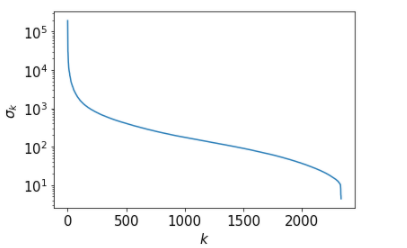
\includegraphics[]{sigma_image.png}
    \caption{The variability of singular values}
\end{figure}
We can see that the singular values decrease quickly at $k = 100$.
\begin{figure}[H]
    \center
    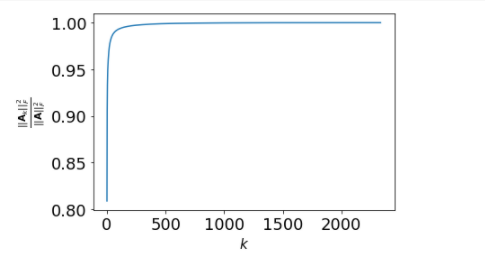
\includegraphics[]{true_ratio.png}
    \caption{Ratio keep image features}
\end{figure}
Above graph represent for ratio keep information from the picture when $k$ change. We can see that at $k = 100$, we can keep almost all the information from the picture.
\begin{figure}[H]
    \center
    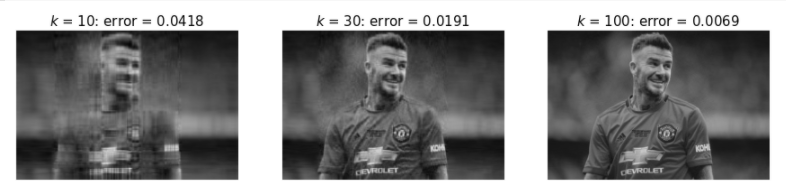
\includegraphics[scale = 0.7]{choose_k.png}
    \caption{Picture got from different k}
\end{figure}

Storing picture with Truncated SVD, we will store matrices $\mathbf{U}_k \in \mathbb{R}^{m \times k}, \Sigma_k \in \mathbb{R}^{k \times k}, \mathbf{V}_k \in \mathbb{R}^{n \times k}$. Total elements we need to store is $k(m + n + 1)$ - notice that we only store $K$ values in the main diagonal line in $\Sigma_k$. Assuming an float element cost 4 bytes, total bytes is $ 4k(m + n + 1)$, original picture cost $ mn $ bytes - intergers cost 1 byte. So compression rate is : $$ \frac{4k(m + n + 1)}{mn} $$
\indent \par When $ k \ll mn $, we got a rate smaller than 1. With our example,choosing $k = 100$,$  m =3500 ,n = 2336$. We got a rate approximately $0.29$, saving 70\% memory.
\chapter{\Large Principal Component Analysis (PCA)}
\indent \par Like Truncated SVD, PCA is a method that reduces the dimension of data and keeps its main features. PCA convert the basis of related variables to the basis of unrelated variables and maximize the variance.
\section{Some probability theory and statistics}
\subsection{Expected value and Variance}
In probability theory:

\textbf{Expected value} of a random variable is the mean of all specific values of it.

\textbf{Variance} is the expectation of the squared deviation of a random variable from its mean.

In 1-dimension data:\\
Given N values $x_1, x_2, \dots, x_N$. Expected value and variance of the data calculated by follow formula:

\begin{equation*}
\bar{x} = \frac{1}{N}\sum_{n=1}^N x_n
\end{equation*}
\begin{equation*}
var(X)=\sigma^2 = \frac{1}{N} \sum_{n=1}^N (x_n - \bar{x})^2
\end{equation*}\\
\indent \par Expected value is simply arithmetic mean of all value in the data. $\sigma$ is standard deviation.

In N-dimension data:\\
\indent \par Given $N$ point of data expressed by column vectors $\mathbf{x}_1, \dots, \mathbf{x}_N$, then our \textbf{expected value vector} is caculated from this formula:
\begin{equation*}
\bar{\mathbf{x}} = \frac{1}{N} \sum_{n=1}^N \mathbf{x}_n \ 
\end{equation*}

\subsection{Covariance and Covariance matrix}

\indent \par In probability theory:

\textbf{Covariance} is a measure of the relationship between random variables. 
$$cov(x,y) = \frac{\sum_{i=1}^{n} (x_i - \hat{x})(y_i - \hat{y})}{N}$$

\textbf{Covariance matrix} is a square matrix with the variance of variables in the diagonal line and the covariance of variables in the other position.

\begin{equation*}
    \mathbf{S} =  \frac{1}{N}\sum_{n=1}^N (\mathbf{x}_n - \bar{\mathbf{x}})(\mathbf{x}_n - \bar{\mathbf{x}})^T = \frac{1}{N}\hat{\mathbf{X}}\hat{\mathbf{X}}^T ~(with~ \hat{\mathbf{X}}=\mathbf{x}_n - \bar{\mathbf{x}})
\end{equation*}\\

\indent Example for covariance matrix of 3 features $X,Y,Z$:

\begin{equation*}
S = \begin{pmatrix} 
var(X) & cov(X,Y) & cov(X,Z)\\
cov(X,Y) & var(Y) & cov(Y,Z)\\ 
cov(X,Y) & cov(Y,Z) & var(Z) 
\end{pmatrix}
\end{equation*}\\
\indent Some features about covariance matrix:
\begin{itemize}
\item Every value in the main diagonal line in the covariance matrix is a non-negative value. It's also a variance in each dimension of the data.
\item Remaining values that are not in the main diagonalize express correlation between the data components also called covariance. These value can be positive, negative or 0.
\item We got data that does not correlate with its components or dimension if we got a diagonal covariance matrix.
\end{itemize}

An example image about correlation or uncorrelation data:
\begin{figure}[H]
    \center
    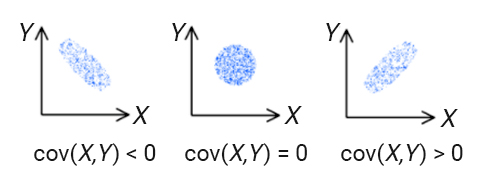
\includegraphics[scale=3]{covx-y.jpg}
\end{figure}

\textbf{The reason to choose covariance matrix to get the principal components of features X in PCA:}
The covariance matrix represents the variation in the data set. The diagonal elements show the scatter of the variables and the correlation between the variables in the other elements. For variables whose value does not change or change insignificantly, we consider that variable does not store too much information. Thus, PCA is converting the original base system to a new one of uncorrelated variables and eliminating the variables with small variances to optimize the amount of information stored. PCA helps reduce the number of initial variables, into some important components, while preserving data.
\section{Into PCA}
\indent \par The idea of PCA is plotting the data into a new basis system. In that system, the importance of the components is significantly different from ignoring the least important component.

From the data X, we will split X into A and B in which the data is mainly concentrated in A, B only carries a small amount of information.

Assume the new orthonormal basis is $U$, and we want to keep $K$ points on this new basis. First, $K$ points plot almost information in the data X. This idea is shown in the below image:
\begin{figure}[H]
    \center
    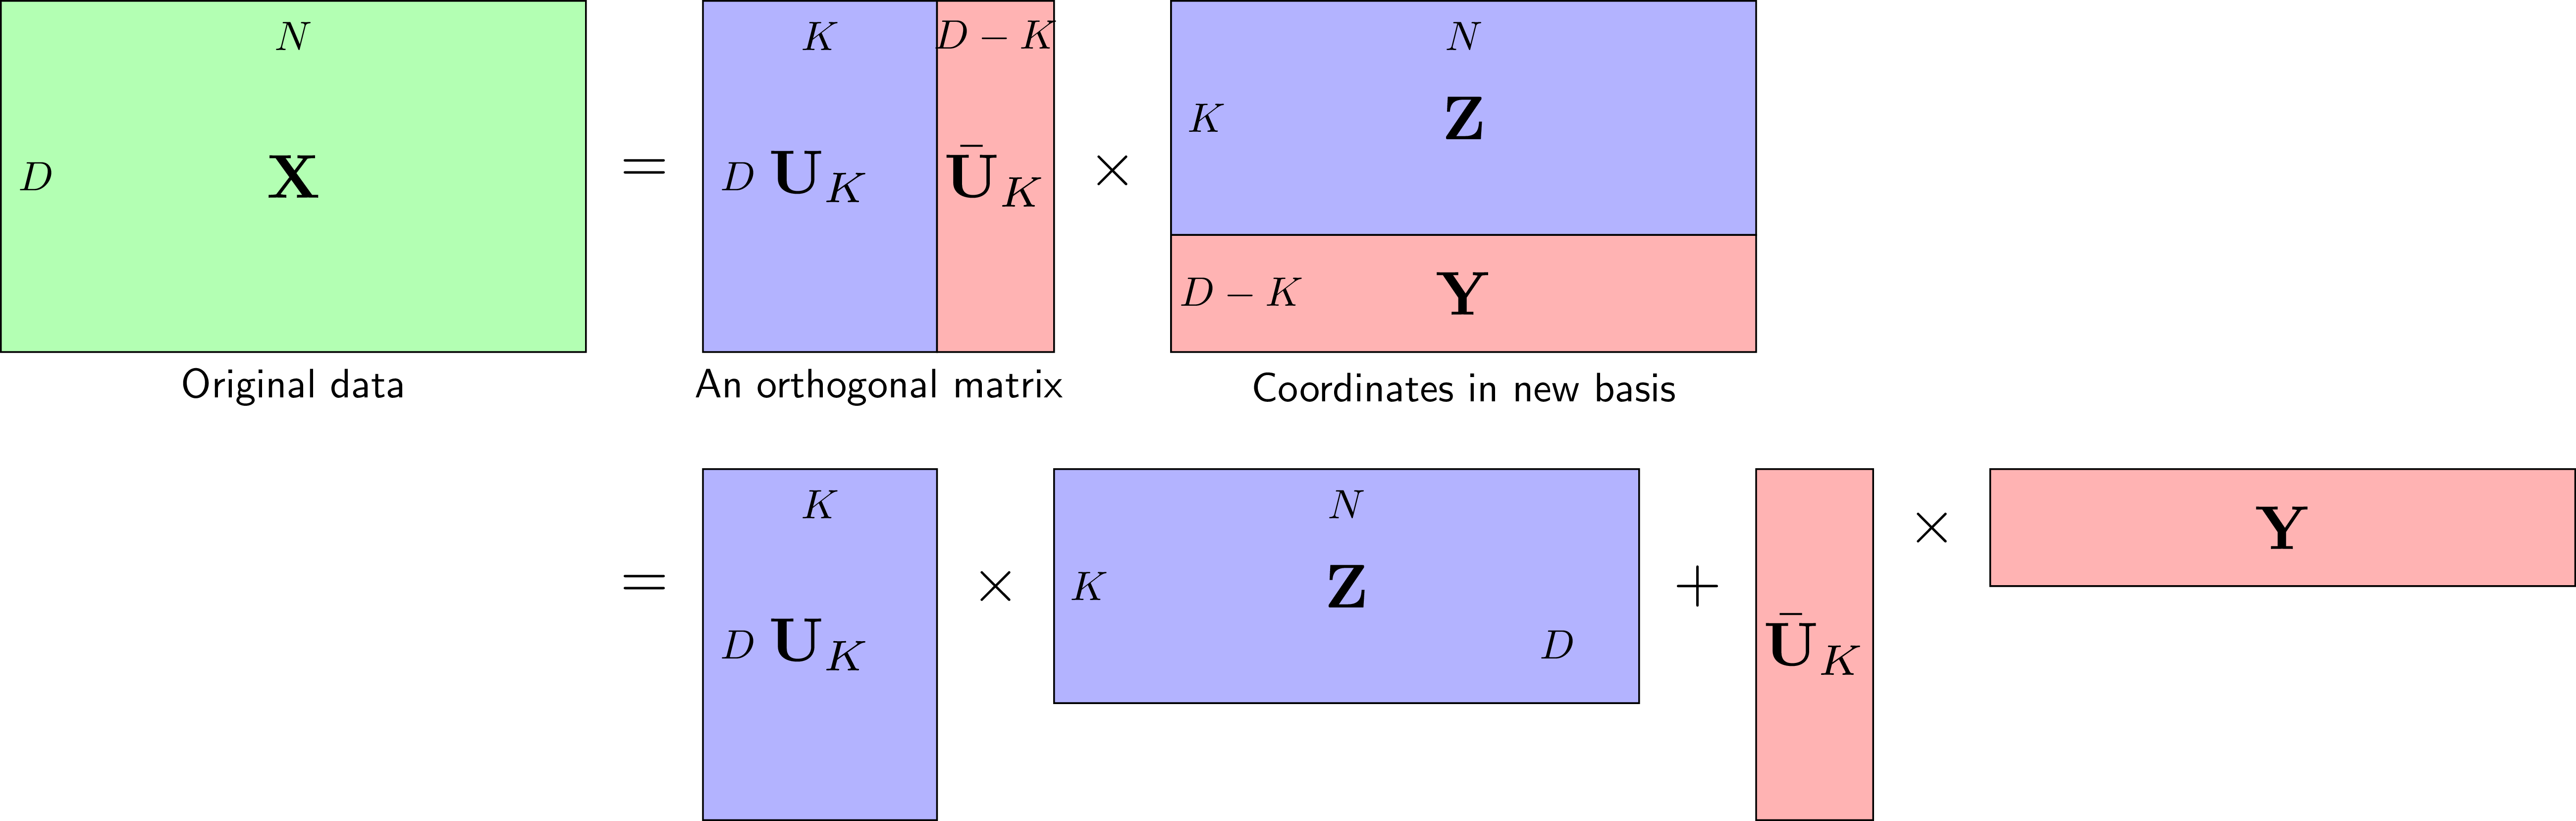
\includegraphics[width=10cm,height=4cm]{pca_idea.png}
    \caption{The PCA idea}
\end{figure}
We having: 
\begin{eqnarray*}
  \mathbf{X} &=& \mathbf{U}_K \mathbf{Z} + \bar{\mathbf{U}}_K \mathbf{Y}\\
  &=& \mathbf{A} + \mathbf{B}
\end{eqnarray*}
\indent with $\mathbf{A} = \mathbf{U}_K \mathbf{Z}, \mathbf{B} =\bar{\mathbf{U}}_K \mathbf{Y}$. Assuming we have $A$, minimizing the loss, we approximate $B$ with a formula :
 $$B=\bar{\mathbf{U}}_K \bar{\mathbf{U}}_K^T\bar{\mathbf{x}}\mathbf{1}^T$$ 
\indent \par We can watch a proof in a blog about basic ML by Vu Huu Tiep \href{https://machinelearningcoban.com/2017/06/15/pca/}{\textcolor{blue}{PCA - machinelearningcoban}}. We got:
 $$\mathbf{X} \approx \tilde{\mathbf{X}} = \mathbf{U}_K \mathbf{Z} + \bar{\mathbf{U}}_K \bar{\mathbf{U}}_K^T\bar{\mathbf{x}}\mathbf{1}^T$$
\indent \par From above formula, we have our loss function:
\begin{eqnarray*}
    L&=& \frac{1}{N} || \mathbf{X} - \tilde{\mathbf{X}}||_F^2 = \frac{1}{N} ||\bar{\mathbf{U}}_K \bar{\mathbf{U}}_K^T \mathbf{X} -  \bar{\mathbf{U}}_K \bar{\mathbf{U}}_K^T \bar{\mathbf{x}}\mathbf{1}^T||_F^2\\
    &=& \frac{1}{N} ||\bar{\mathbf{U}}_K \bar{\mathbf{U}}_K^T \mathbf{X} -   \bar{\mathbf{x}}\mathbf{1}^T||_F^2 \  \\
    &=& \frac{1}{N} || \bar{\mathbf{U}}_K^T (\mathbf{X} -   \bar{\mathbf{x}}\mathbf{1})^T||_F^2 ~~~(\bar{\mathbf{U}}_K\,\, orthonormal)  \  \\
    &=&  \frac{1}{N} ||\hat{\mathbf{X}}^T \bar{\mathbf{U}}_K ||_F^2 = \frac{1}{N} ||\bar{\mathbf{U}}_K^T\hat{\mathbf{X}} ||_F^2  \\
    & = & \frac{1}{N}\sum_{i = K+1}^D ||\hat{\mathbf{X}}^T\mathbf{u}_i ||_2^2\\
    &=& \sum_{i=K+1}^D \mathbf{u}_i^T\mathbf{S} \mathbf{u}_i~~(S=\hat{\mathbf{X}}\hat{\mathbf{X}}^T)
\end{eqnarray*}
\indent \par After that, we optimize the loss function $L$ :

\begin{eqnarray*}
    L&=&\sum_{i=k+1}^D \mathbf{u}_i^T\mathbf{Su}_i = \frac{1}{N-k} ||\hat{\mathbf{X}}^T\bar{\mathbf{U}}_K||_F^2\\
    &=& \frac{1}{N-k} \text{trace}(\hat{\mathbf{X}}^T\bar{\mathbf{U}}_K \bar{\mathbf{U}}_K^T \hat{\mathbf{X}})~~~(\bar{\mathbf{U}}_K\,\, orthonormal) \\ 
    &=& \frac{1}{N-k} \text{trace} (\hat{\mathbf{X}}^T \hat{\mathbf{X}})= \frac{1}{N-k} \text{trace} (\hat{\mathbf{X}} \hat{\mathbf{X}}^T) \\ 
    &=& \text{trace} (\mathbf{S}) = \sum_{i=k+1}^D \lambda_i~ (With ~\lambda_i \geq 0)\\
\end{eqnarray*}
\indent \par $L$ do not depend on $U$. Function $L$ minimized $\Leftrightarrow$From $k+1$ to $D$, we have $D-k$ minimum eigenvalues of the covariance matrix. In the other words, we have the $k$ biggest eigenvalues of the covariance matrix $S$ and $u_i$ is the $k$ eigenvectors correspondingly to those eigenvalues.\\
Conclusion, PCA helps us to reduce dimension the basis system for the original data but still retain most of the information. ( From $D$ to $K$ with $K \ll D$).



\section{Step By Step Computation Of PCA}
\textbf{Having 7 steps to compute of PCA}\\
Step 1: Find mean vector
\begin{eqnarray*}
\bar{x} &=& \frac{1}{N}\sum_{n=1}^N x_n
\end{eqnarray*}
Step 2: Subtract mean
\begin{eqnarray*}
\hat{\mathbf{x}}_n = \mathbf{x}_n - \bar{\mathbf{x}}
\end{eqnarray*}
Step 3: Calculate the covariance matrix for the features in the dataset
\begin{eqnarray*}
\mathbf{S} = \frac{1}{N}\hat{\mathbf{X}}\hat{\mathbf{X}}^T
\end{eqnarray*}
Step 4: Calculate eigenvalues, eigenvector and sort those eigenvalues in ordered descending (These eigenvector must be normalized)\\
Step 5:  Pick $K$ eigenvector $u$ corresponding to the $K$ highest eigenvalues\\
Step 6: Project data to selected eigenvector
\begin{eqnarray*}
\mathbf{Z} = \mathbf{U}_K^T\hat{\mathbf{X}}
\end{eqnarray*}
We can approximate the original data by doing:
$$\mathbf{x} \approx \mathbf{U}_K\mathbf{Z} + \bar{\mathbf{x}}$$
For large datasets, we need to add the data normalization step before performing the above steps. Skipping the data normalization step can greatly affect the results. \\
It can be calculated like so:
$$ x = \frac{variable ~ value - mean}{standard ~ deviation}$$
\begin{figure}[H]
    \center
    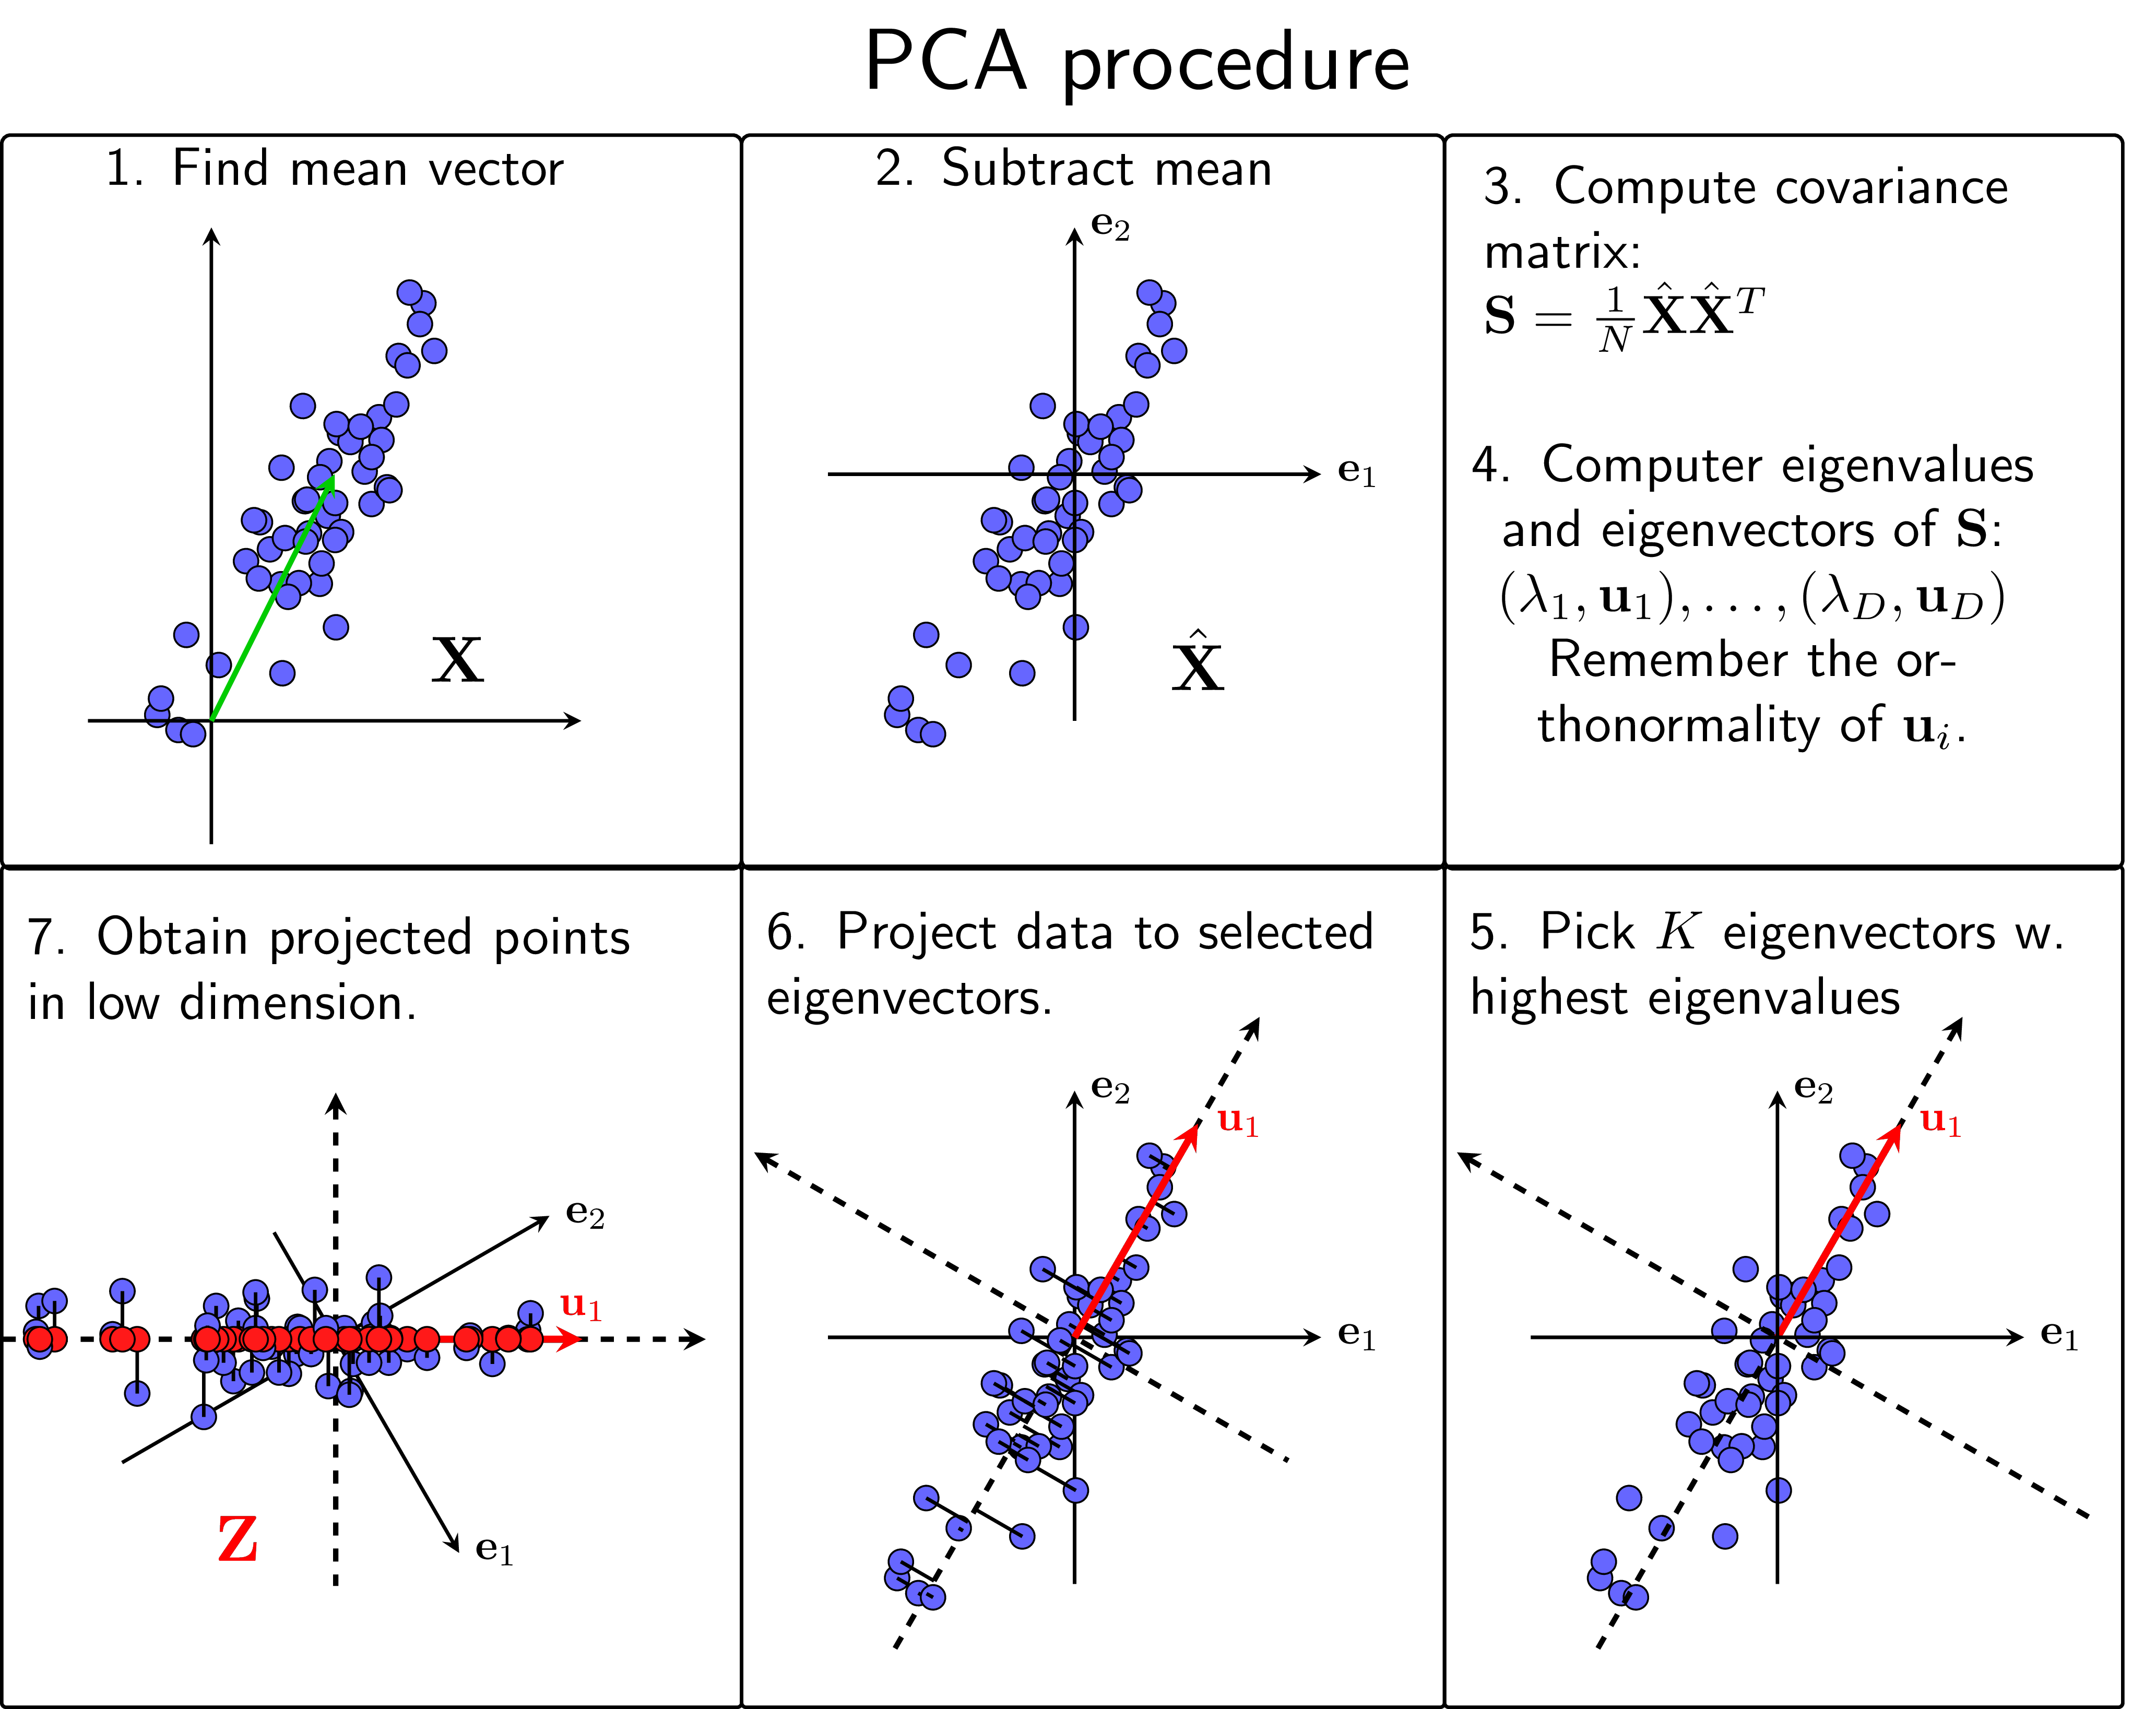
\includegraphics[width=10cm,height=8cm]{pca_procedure.png}
    \caption{Step by step explanation of PCA}
\end{figure}
\textbf{Running example PCA:}\\
Given the following data, use PCA to reduce the dimension from 2 to 1
\begin{center}
 \begin{tabular}{||c|c|c|c|c||} 
 \hline
 Feature & Example1 & Example2 & Example3 & Example4 \\ [0.5ex] 
 \hline\hline
 x & 4 & 8&13 & 7 \\ 
 \hline
 y & 11 & 4 & 5&14 \\
 \hline

\end{tabular}
\end{center}
$$\Rightarrow X=\begin{pmatrix} 4 & 8 & 13 & 7\ \\ 11 & 4 & 5 & 14 \end{pmatrix}$$\\
\indent Step 1: Find mean vector
\begin{itemize}
    \item Number of features, m=2
    \item Number of samples, n=4
\end{itemize}

\begin{eqnarray*}
\bar{x} &=& \frac{1}{N}\sum_{n=1}^N x_n\\
\Leftrightarrow \bar{x}&=&\begin{bmatrix} 8\\ 8.5 \end{bmatrix}
\end{eqnarray*}
\indent Step 2: Subtract mean
$$\hat{\mathbf{x}}_n = \mathbf{x}_n - \bar{\mathbf{x}}$$\
$$\Rightarrow \hat{X}=\begin{pmatrix} -4 & 0 & 5 & -1\ \\ 2.5 & -4.5 & -3.5 & 5.5 \end{pmatrix}$$
\indent Step 3: Calculate the covariance matrix for the features in the dataset
\begin{eqnarray*}
    \mathbf{S} &=& \frac{1}{N}\hat{\mathbf{X}}\hat{\mathbf{X}}^T\\
    &=& \begin{pmatrix} var(x) & cov(x,y)\ \\ cov(y,x) & var(y)  \end{pmatrix}\\
    &=& \begin{pmatrix} 14 & -11\ \\ -11 & 23  \end{pmatrix}
\end{eqnarray*}\\
\indent Step 4: Calculate eigenvalues, eigenvector and sort those eigenvalues in ordered descending (These eigenvector must be normalized)\\
\begin{eqnarray*}
det(S - \lambda I ) &=& 0\\
\lambda^2 - 37\lambda + 201&=&  0\\
\Rightarrow \lambda &=& 30.3849 ~~~ or ~~~ \lambda  =  6.6151   
\end{eqnarray*}
\indent With  $\lambda$ = 30.3849 (this is the first principal component) 
\begin{eqnarray*}
    (S - \lambda I) u_1 &=& 0\\
    \begin{pmatrix} 14- \lambda&-11\\ -11 & 23 - \lambda \end{pmatrix}\begin{bmatrix} u_{11}\\ u_{12} \end{bmatrix}&=&\begin{bmatrix} 0\\ 0 \end{bmatrix}\\
    \Rightarrow u_1&=& \begin{bmatrix} 11\\ -16.3849 \end{bmatrix}
\end{eqnarray*}\\
\indent Normalizing $u_1$ we got:
$$  u_1 = \begin{bmatrix} 0.5574\\ -0.8303 \end{bmatrix} $$\\
\indent Step 5:  Pick K eigenvector w. highest eigenvalues

\indent Because the data has only 2 dimension so we skip this step.\\
\indent Step 6: Project data to selected eigenvector.

$$  p_{11} = u_1^T\begin{bmatrix} -4\\ 2.5 \end{bmatrix} =-4.3052$$

$$  p_{12} = u_1^T\begin{bmatrix} 0\\ -4.5 \end{bmatrix} =3.7361$$

$$  p_{13} = u_1^T\begin{bmatrix} 5\\ -3.5 \end{bmatrix} =5.6928$$

$$  p_{14} = u_1^T\begin{bmatrix} -1\\ 5.5 \end{bmatrix} =-5.1238$$


\indent Step 7: Reducing the dimensions of the data set
\begin{eqnarray*}
\mathbf{Z} = \mathbf{U}_K^T\hat{\mathbf{X}}
\end{eqnarray*}
\begin{center}
 \begin{tabular}{||c|c|c|c|c||} 
 \hline
 Feature & Example1 & Example2 & Example3 & Example4 \\ [0.5ex] 
 \hline
 PC1 & -4.3052 & 3.7361&5.6928 & -5.1238 \\ 
\hline

\end{tabular}
\end{center}

\section{Relationship between PCA and SVD} 
\indent \par The data has been preprocessed to have zero mean.
\begin{eqnarray*}
\Rightarrow  S=\frac{1}{n}\mathbf X\mathbf X^\top
\end{eqnarray*}
\par Cause S is a symmetric matrix, eigenvectors of S are orthogonal. Therefore, we normalize that eigenvectors and they will be orthonormal.
$$S=\frac{1}{n}\mathbf U\mathbf D\mathbf U^\top~~~(1)$$
\par On the other hand, when implementing SVD, we have:
\begin{eqnarray*}
S &=&\frac{1}{n}\mathbf X\mathbf X^\top
=\frac{1}{n}(\mathbf U\mathbf \Sigma\mathbf V^\top)(\mathbf U\mathbf \Sigma\mathbf V^\top)^\top
= \frac{1}{n}(\mathbf U\mathbf \Sigma\mathbf V^\top)(\mathbf V\mathbf \Sigma\mathbf U^\top)\\
&=&\frac{1}{n}\mathbf U\mathbf \Sigma^2 \mathbf U^\top ~~~(\bar{\mathbf{U}}\,\, orthonormal) ~~~(2)
\end{eqnarray*}
\par From (1) and (2), U after diagonalize covariance matrix is the same as when we factorize matrix by using SVD.
\par We can approximate matrix by using Truncated SVD:
$$\mathbf{X} \approx \tilde{\mathbf{X}} = \mathbf{U}_K \mathbf{\Sigma}_K \mathbf{V}_K^T~~~(3)$$
\par When we approximate by using PCA:
$$\mathbf{X} \approx \tilde{\mathbf{X}} = \mathbf{U}_K \mathbf{Z}~~~(4)$$
\par From (3) and (4), $U_k$ in truncated SVD is the same as $U_k$ in PCA and 
$ \mathbf{\Sigma}_K \mathbf{V}_K^T$ in truncated SVD is $Z$ in PCA.

\section{PCA for large-scale problems}

\indent \par In practice, the number of data points $N$, and its dimensions $D$ are so large. Therefore, we have to find eigenvalues for a huge matrix. E.g. we have 1 Million images containing $1000 \times 1000$ pixels, so we have $D = 10^6 = N$, and it is difficult and time-consuming to find eigenvalues for a covariance matrix that is calculated from $10^6 \times 10^6$ matrix. However, we have a method to find that approximately eigenvalues quickly called \textbf{Power Method}.

To find eigenvalues and eigenvectors for a positive semi-definite matrix $\mathbf{A} \in \mathbb{R}^{n \times n}$:
\begin{itemize}
\item Step 1: Choose a random vector $\mathbf{q}^{(0)} \in \mathbb{R}^n, ||\mathbf{q}^{(0)}||_2 = 1$ and $k = 1$
\item Step 2: Calculate $\mathbf{z} = \mathbf{Aq}^{(k-1)}$
\item Step 3: Normalize $\mathbf{q}^{(k)} = \frac{\mathbf{z}}{||\mathbf{z}||_2}$
\item Step 4: While $||\mathbf{q}^{(k)} - \mathbf{q}^{(k-1)}||_2 < \epsilon
$ then stop, else $k = k + 1$ and return to step 2.
\end{itemize}

Now we have largest eigenvalue $\lambda_1 = (\mathbf{q}^{(k)})^T\mathbf{A}\mathbf{q}^{(k)}$ and corresponding eigenvector $\mathbf{q}^{(k)}$. Let prove this method:
If $A$ is a positive semi-definite matrix then there exist $n$ independent eigenvectors of $A$. Let $x_1,...,x_n$ be these eigenvectors, then $x_1,...,x_n$ form a basis of $\mathbb{R}^n$. Hence the initial vector $q^{(0)}$ can be written as: $q^{(0)} = a_1x_1 + a_2x_2 + ... + a_nx_n$ where $a_1,..., a_n$ are scalars.

Multiplying both sides of the equation in $A^k$ yields:
\begin{eqnarray*}
A^kq^{(0)} &=& A^k(a_1x_1 + a_2x_2 + ... + a_nx_n) \\
&=& a_1A^kx_1 + a_2A^kx_2 + ... + a_nA^kx_n \\
&=& a_1\lambda_1^kx_1 + a_2\lambda_2^kx_2 + ... + a_n\lambda_n^kx_n \\
&=& a_1\lambda_1^k(x_1 +\sum_{j=2}^{n}\frac{a_j}{a_1}(\frac{\lambda_j}{\lambda_1})^kx_j)  
\end{eqnarray*}

If $|\lambda_1| > |\lambda_2| \geq \dots \geq |\lambda_n| \geq 0$ then we say that $\lambda_1$ is a dominant eigenvalue. In this case $(\frac{\lambda_j}{\lambda_1})^k \to 0$ and therefore if $a_1 \neq 0, A^kq^{(0)} \to a_1\lambda_1^kx_1$. The power method normalizes the products $Aq^{(k-1)}$ to avoid overflow, therefore it converges to $x_1$.

To find the next eigenvalue and eigenvector, we have a matrix $\mathbf{B} = \mathbf{A} - \lambda_1 \mathbf{v}_1 \mathbf{v}_1^T$ that have eigenvalues $\lambda_2 \geq \lambda_3 \geq \dots \geq \lambda_n \geq 0$ and corresponding eigenvectors $\mathbf{v}_2, \mathbf{v}_3, \dots, \mathbf{v}_n$.

Prove it by using inductive method:
\begin{itemize}
    \item With $i = 1$: 
        \begin{eqnarray*}\mathbf{Bv}_1 = (\mathbf{A} - \lambda_1 \mathbf{v}_1\mathbf{v}_1^T) \mathbf{v_1} = \mathbf{Av}_1 - \lambda_1 \mathbf{v}_1 = \mathbf{0} 
        \end{eqnarray*}
    \item With $i > 1$:
        \begin{eqnarray*}
        \mathbf{Bv}_i = (\mathbf{A} - \lambda_1 \mathbf{v}_1 \mathbf{v}_1^T)\mathbf{v}_i = \mathbf{Av}_i - \lambda_1 \mathbf{v}_1 (\mathbf{v}_1^T \mathbf{v}_i) = \mathbf{Av}_i = \lambda_i \mathbf{v}_i
        \end{eqnarray*}
\end{itemize}



Hence, $(\lambda_2, \mathbf{v}_2)$ has became a large pair of eigenvalue and eigenvector of $\mathbf{B}$. Therefore, we can find this pair by using Power method for $\mathbf{B}$. Repeat this process, we can find up to eigenvalue $\mathbf{K}-th$ for covariance matrix.

\section{Some notice when calculating PCA in real data} 
\indent \par There are two cases that we need to notice when calculating PCA in reality. First, the data is much smaller than the dimension of the data. Second, the training data is huge, can up to millions. The covariance matrix and eigenvalue calculation can be impossible. We still have solutions for those cases.

This section assumes that the data has been normalized, which the expected vector subtracts the data. Then, the covariance matrix will be calculated by this formula: $\mathbf{S} = \frac{1}{N}\mathbf{X}\mathbf{X}^T$.
\subsection{Dimensions of the data is bigger than datapoints}
\indent \par When $D > N$, eigenvalues of the covariance matrix $S$ will not larger than N. So we need to pick $K \leq N$ cause we can't pick $ K > N $ non-zero eigenvalue of a rank-$N$ matrix.

\indent \par Calculating eigenvalues and eigenvectors can be be effectively implemented if we follow these features: 
\begin{itemize}
\item Eigenvalues of $A$ is equal to eigenvalues of $kA$ with non-zero $k$
\item Eigenvalues of $\mathbf{AB}$ is equal to eigenvalues of $\mathbf{AB}$ with $ \mathbf{A} \in \mathbb{R}^{d_1 \times d_2}, \mathbf{B} \in \mathbb{R} ^{d_2 \times d_1} $ and $d_1, d_2$ is a non-zero number. 
\indent \par Instead of finding eigenvalue in covariance matrix $\mathbf{S} \in \mathbb{R}^{D\times D}$, we can find eigenvalue matrix $\mathbf{T} = \mathbf{X}^T \mathbf{X} \in \mathbb{R}^{N \times N} $ having smaller dimension ($N < D$)
\item Assuming $\mathbf{T} = \mathbf{X}^T \mathbf{X} \in \mathbb{R}^{N \times N}$ is a pair of eigen value-vector of $\mathbf{T} $ then $(\lambda, \mathbf{Xu})$is a pair of eigen value-vector of  $\mathbf{S}$. Proof: \begin{eqnarray*}
  \mathbf{X}^T \mathbf{Xu} = \lambda \mathbf{u} \Rightarrow (\mathbf{X}\mathbf{X}^T)(\mathbf{Xu}) = \lambda \mathbf{Xu}
\end{eqnarray*}
\end{itemize}

\subsection{Normalization EigenVectors}
\indent \par \textit{Recall the definition of eigenspace: The eigenspaces corresponding to the eigenvalues of a matrix are the span subspace created by all the eigenvectors corresponding to that eigenvalue.}

\indent \par The last thing to do in PCA is normalizing eigenvectors so that they form an orthonormal system. This can be based on the following two points:
\begin{itemize}
    \item First,if $\mathbf{A}$ is a symmetric matrix, $(\lambda_1, \mathbf{x}_1), (\lambda_2, \mathbf{x}_2)$ is pairs of eigenvalue-eigenvector of A, then $\mathbf{x}_1^T\mathbf{x}_2 = 0$. In other words, any two vectors in two different eigenspaces of a symmetrical matrix are perpendicular to each other. Proof: 
\begin{eqnarray*}
  \mathbf{x}_2^T \mathbf{Ax}_1 = \mathbf{x}_1^T \mathbf{Ax}_2 = \lambda_1 \mathbf{x}_2^T \mathbf{x}_1 = \lambda_2 \mathbf{x}_1^T \mathbf{x}_2 \Rightarrow \mathbf{x}_1^T \mathbf{x}_2 = 0 ~~~~~ cause ~~~\lambda_1 \neq \lambda_2 
\end{eqnarray*}
\item Second, with independent eigenvalues found in eigenspaces, we can use the Gram-Schmit process to normalize them into an orthonormal system.
\end{itemize}
\indent \par Combining two points above, we can obtain the individual vectors to form an orthonormal system, which is the matrix $\mathbf{U}_K$ in PCA.



\section{Application and Example of PCA} 
\subsection{PCA in analysis data}

\indent \par PCA is a great tool for analyzing high-dimensional data. We gonna create 2d data with Gaussian distribution. So we can try to analyze the data for understanding the dominant direction of variants in that data.
\begin{minted}[frame=lines,framesep=2mm,baselinestretch=1.2]{python}
import numpy as np

xC = np.array([2.5,0.5]) #center of data (mean)
sig = np.array([2.5,0.5]) #principal axes

theta = np.pi/3

R = np.array([[np.cos(theta), -np.sin(theta)], 
              [np.sin(theta),np.cos(theta)]])  #rotaion matrix
nPoints = 10000  #creating 10k points
X = R .dot(np.diag(sig)).dot(np.random.randn(2,nPoints))
+ np.diag(xC).dot(np.ones((2,nPoints)))
\end{minted}
\begin{figure}[H]
    \center
    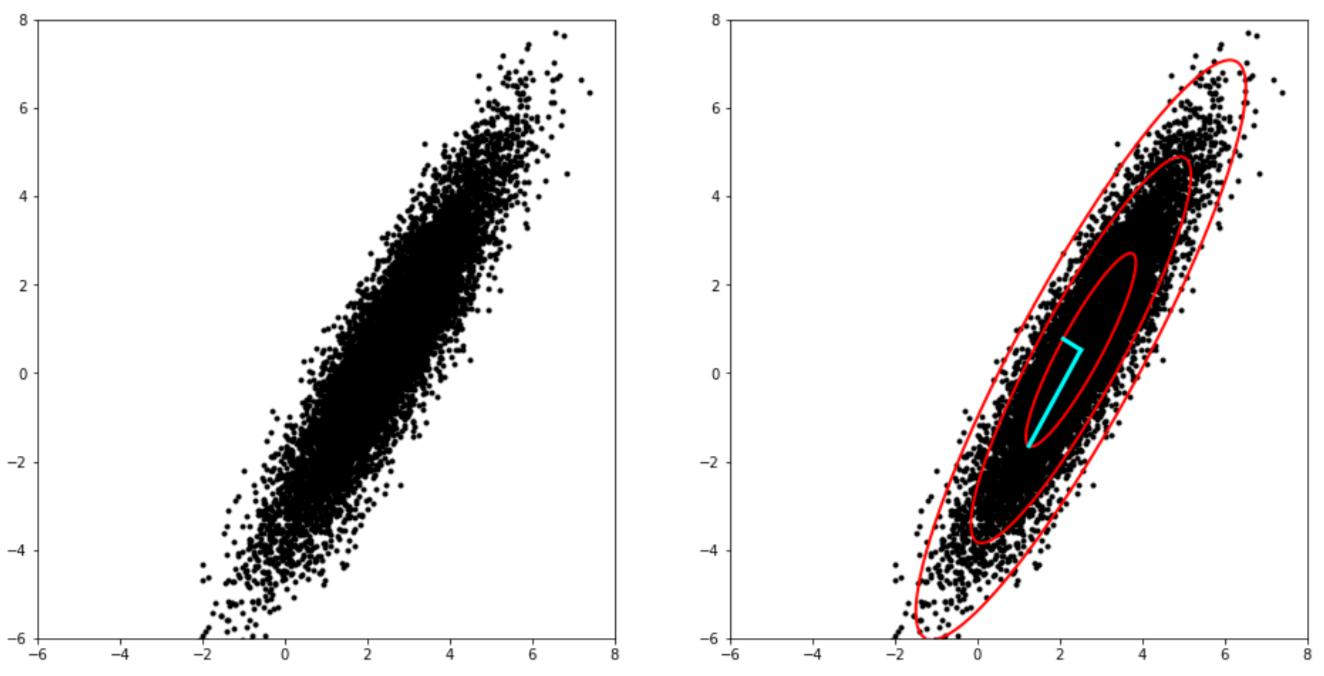
\includegraphics[width=15cm,height=7.5cm]{pca1.jpg}
    \caption{Plotting 10000 points and its standard deviation.}
\end{figure}
\indent \par After plotting the data and its principal components. We can see singular values in $\Sigma$ almost 2.5 and 0.5. The first principal components direction has a lot of variance of 2 and the second components have a small variance of 0.5. In the $U$ matrix, we can know how the data is rotated. The first column in $U$ is the rotated first principal components direction, the same with the second column.
3 ellipse is represented for 3 standard deviation ellipse. We can know how much standard deviation a data point has.

\subsection{Eigenfaces for face recognition}
\indent \par Eigenfaces is one of the most popular methods for facing recognition. This method's idea is finding a vector space that has a small dimension than the original space. Then, we can use these vectors as the feature vectors to projecting data for classification. Actually, eigenfaces are eigenvectors corresponding to the largest eigenvalues of the covariance matrix in PCA. As an example, we use the Labeled Faces in the Wild dataset to do an eigenfaces test.

The picture below is the first 10 pictures in the dataset.
\begin{figure}[H]
    \center
    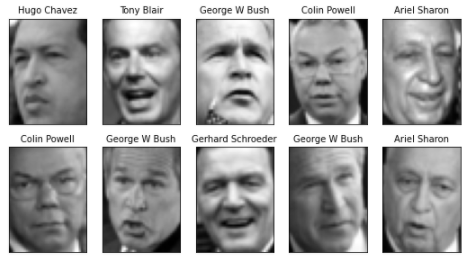
\includegraphics[width=15cm,height=7.5cm]{face_demo.png}
    \caption{First 10 pictures in the dataset}
\end{figure}
The dataset that we used has $1288$ samples and $1850$ dimensions. This means every sample has the size of $50 \times 37$.
\begin{minted}[frame=lines,framesep=2mm,baselinestretch=1.2]{python}
from sklearn.decomposition import PCA
n_components = 150
pca = PCA(n_components, svd_solver='randomized',whiten=True)
pca.fit(X)
eigenfaces = pca.components_.reshape((n_components, h, w))
U = pca.components_.T
\end{minted}
\begin{figure}[H]
    \center
    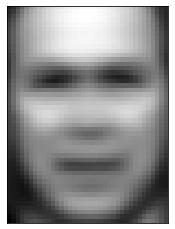
\includegraphics{meanface.jpg}
    \caption{Eigenface mean}
\end{figure}
\begin{figure}[H]
    \center
    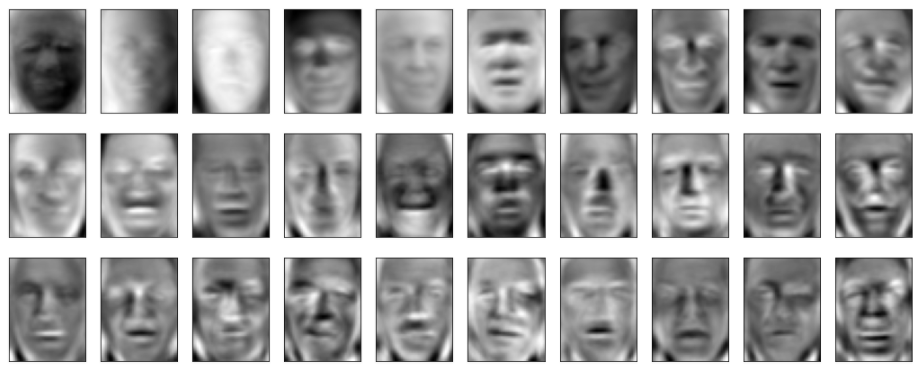
\includegraphics[scale = 0.6]{eigenfaces.png}
    \caption{First 30 eigenfaces}
\end{figure}

This is the result after we were projecting data on eigenfaces space and approximating that.

\begin{figure}[H]
    \center
    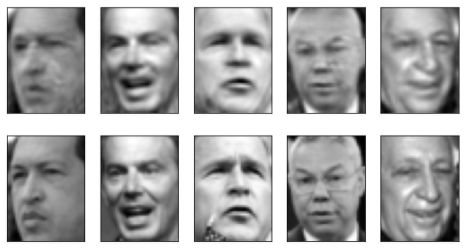
\includegraphics[scale=0.8]{face_appr.png}
    \caption{First 5 face approximated on eigenfaces}
\end{figure}


\subsection{Eigengene in human gene data}
\indent \par We gonna analyze an Ovarian cancer data (a built data) - 216 individual patients with 4000 genetic markers that are measured for every patient. These patients are broken into two groups. The first half has cancer, and the second half has no cancer. We are gonna use PCA to decompose this high dimensional data. After that, we are gonna visualize the data in 3D, find the relationship of the variables.
\begin{figure}[H]
    \center
    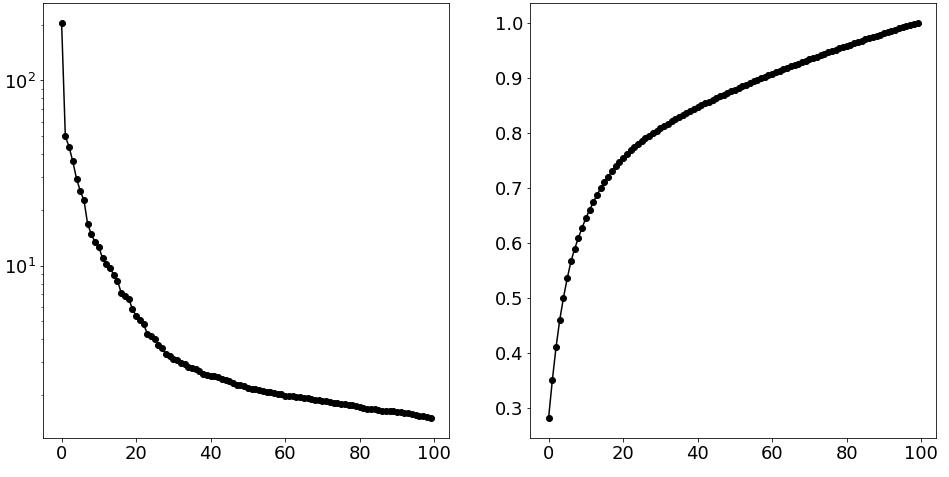
\includegraphics[width=15cm,height=7.5cm]{pca2-2.jpg}
    \caption{First K of eigenvalues and}
\end{figure}
\indent \par First plot is plotting the eigen values in $\Sigma$. The second plot is result of dividing cumulative sum and the sum of eigen values in $\Sigma$, it represents how much variance is captured by first $k$ eigen values $${\frac{\sum_{i=1}^k \sigma_i^2}{\sum_{j = 1}^r \sigma_j^2}}$$

The first plot is plotting the eigenvalues in $\Sigma$. The second We can see in the first plot. Only about the first 25 eigenvalues is considerable large. After 50 eigenvalues, the value is slowly decreasing. This means only the first 25 eigenvalues contain a big variance of the dataset, capturing lots of information about our dataset. In the second plot, dividing cumulative sum and the sum of eigenvalues of the first 2 eigenvalues is more than 0.6 -  we know that the first 2 eigenvalues capture more than 60\% the information of the dataset.
\begin{figure}[H]
    \center
    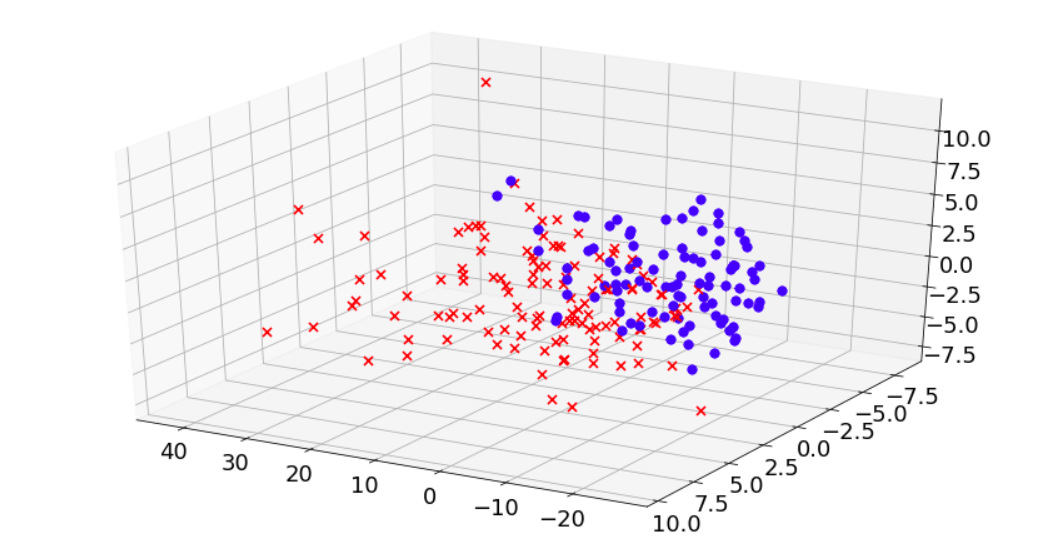
\includegraphics[width=15cm,height=7.5cm]{3eigengenes.png}
    \caption{Plotting 216 patients in first 3 principal components}
\end{figure}
\indent \par In this plot, red x marks represent cancer patients, and blue dots represent non-cancer patients. We can see cancer patients cluster in an area on the left side, the same with non-cancer patients, but they cluster on the right side. So our cancer or non-cancer patients have a relation in the gene data.

\chapter{\LARGE Conclusion}
\indent \par After diving into SVD and PCA, we know that these techniques are powerful for analyzing, reducing high dimensional data. And we also can use these techniques for classifying and compressing data. Besides the advantages of these techniques, it does have drawbacks: information loss, becoming less interpretable. In general, Principal Components Analysis and Singular Value Decomposition is great to use in any situation when working which big data.

\begin{thebibliography}{9}
\bibitem{mlcbebook} 
Machine Learning Co Ban - Tiep Huu Vu.
\\ \href{https://github.com/tiepvupsu/ebookMLCB}{Machine Learning Co Ban Ebook: \texttt{https://github.com/tiepvupsu/ebookMLCB}}
\bibitem{datadriven} 
Data-driven Science and Engineering: Machine Learning, Dynamical System, and Controls - Steven L. Brunton, J. Nathan Kutz.
\\
\href{http://databookuw.com/}{Website and Ebook: \texttt{http://databookuw.com/}} \\
\href{https://github.com/dynamicslab/databook_python}{Data Github:    \texttt{https://github.com/dynamicslab/databook\_python } }
\bibitem{princeton} 
SVD Chapter - Princeton Computer Science Course.
\href{https://www.cs.princeton.edu/courses/archive/spring12/cos598C/svdchapter.pdf}{\\https://www.cs.princeton.edu/courses/archive/spring12/cos598C/svdchapter.pdf}
\bibitem{powermethod} 
Power Method: \href{https://www.cs.huji.ac.il/~csip/tirgul2.pdf}{ \texttt{https://www.cs.huji.ac.il/~csip/tirgul2.pdf}}
\bibitem{gram} 
Gram-Schmidt:
\href{https://ocw.mit.edu/courses/mathematics/18-06sc-linear-algebra-fall-2011/least-squares-determinants-and-eigenvalues/orthogonal-matrices-and-gram-schmidt/MIT18_06SCF11_Ses2.4sum.pdf}{\\https://ocw.mit.edu/courses/mathematics/18-06sc-linear-algebra-fall-2011/least-squares-determinants-and-eigenvalues/orthogonal-matrices-and-gram-schmidt/MIT18\_06SCF11\_Ses2.4sum.pdf}
\bibitem{colab} 
Demonstrate in Google Colab:\\ \href{https://colab.research.google.com/drive/1nTS87DJv-XmnvqKOX_njJ1XhSN6RoVhQ}{https://colab.research.google.com/drive/1nTS87DJv-XmnvqKOX_njJ1XhSN6RoVhQ}
\end{thebibliography}



\end{document} 

